
\subsection{Case IV : Partition Coefficient}

This analysis investigated the sensitivity of repository performance
to the elemental partition coefficient. 

The partition or distribution coefficient, $K_d$, relates the amount of contaminant adsorbed into the 
solid phase of the host medium to the amount of contaminant adsorbed into the 
aqueous phase of the host medium. It is a common empirical coefficient used to 
capture the effects of a number of retardation mechanisms. The coefficient 
$K_{d,i}$, in units of $[m^3\cdot kg^{-1}]$, is the ratio of the mass of 
contaminant $i$ in the solid to the mass of contaminant $i$ in the solution.

As indicated in Table \ref{tab:Cases}, the parameters in this model were all set 
to the default values except a multiplier applied to the expect partitioning 
coefficients, $\langle K_{d,i} \rangle$, for each isotope $i$. This multiplier 
preserved, in some sense, the widely varying 
relative sorption behavior among elements. 

The expected inverse relationship between the partition coefficient resulting 
peak annual dose was found for all elements that were not assumed to be 
effectively infinitely soluble.  It is clear from Figure \ref{fig:KdSum} that 
for partition coefficients greater than a threshold, approximately 
  $1\pm10[m^3\cdot kg^{-1}]$ the relationship between 
peak annual dose and partition coefficient is a strong inverse one. 

\begin{figure}[ht]
  \centering
  \includegraphics[width=\linewidth]{./images/Partitioning_Summary.eps}
  \caption{$K_d$ sensitivity.  The peak annual dose due to an inventory, 
  $N$, of each isotope.}
  \label{fig:KdSum}
\end{figure}

